\documentclass[aos]{imsart}

\RequirePackage{amsthm,amsmath,amsfonts,amssymb}
\RequirePackage[authoryear]{natbib}
\RequirePackage{graphicx}
\RequirePackage{booktabs}
\RequirePackage[UTF8,fontset=fandol]{ctex}
\RequirePackage{xcolor}
\definecolor{CrossRefBlue}{HTML}{1F5AA6}
\definecolor{CitationTeal}{HTML}{007C83}
\definecolor{UrlPurple}{HTML}{7A3E9D}
\RequirePackage[
  unicode=true,
  colorlinks=true,
  linkcolor=CrossRefBlue,
  citecolor=CitationTeal,
  urlcolor=UrlPurple
]{hyperref}

\startlocaldefs
\numberwithin{equation}{section}
\endlocaldefs

% 以下命令由 R 自动生成，不要手工复制数值。
\newcommand{\SampleSize}{32}
\newcommand{\ModelRsquared}{0.827}
\newcommand{\WeightEstimate}{-3.878}


\begin{document}

\begin{frontmatter}
\title{使用 R 与 LaTeX 建立可复现的统计工作流}
\runtitle{R 与 LaTeX 可复现工作流}

\begin{aug}
\author[A]{\fnms{课程}~\snm{示例}}
\address[A]{统计学课程项目}
\end{aug}

\begin{abstract}
本教学示例说明如何用一个 R 入口生成统计论文所需的数值、矢量图和
LaTeX 表格。修改分析并重新运行后，中英文论文会读取同一批最新结果。
\end{abstract}

\begin{keyword}
\kwd{可复现研究}
\kwd{R}
\kwd{LaTeX}
\kwd{相对路径}
\end{keyword}
\end{frontmatter}

\section{引言}

可复现的统计工作应把数据处理、模型估计和论文报告连接起来
\citep{wickham2014}。回归结果还需要保留模型假设与计算来源
\citep{gelman2020}。

\section{方法}

本例使用 R 内置的 \texttt{mtcars} 数据，拟合模型
\(\texttt{mpg} \sim \texttt{wt} + \texttt{hp}\)。R 脚本把论文需要的
结果全部写入项目内部的 \texttt{outputs} 目录。

\section{结果}

分析包含 \SampleSize{} 个观测，模型的 \(R^2=\ModelRsquared\)。
控制马力后，重量每增加 1000 磅，预测每加仑英里数的变化为
\WeightEstimate{}。

\begin{figure}[htbp]
  \centering
  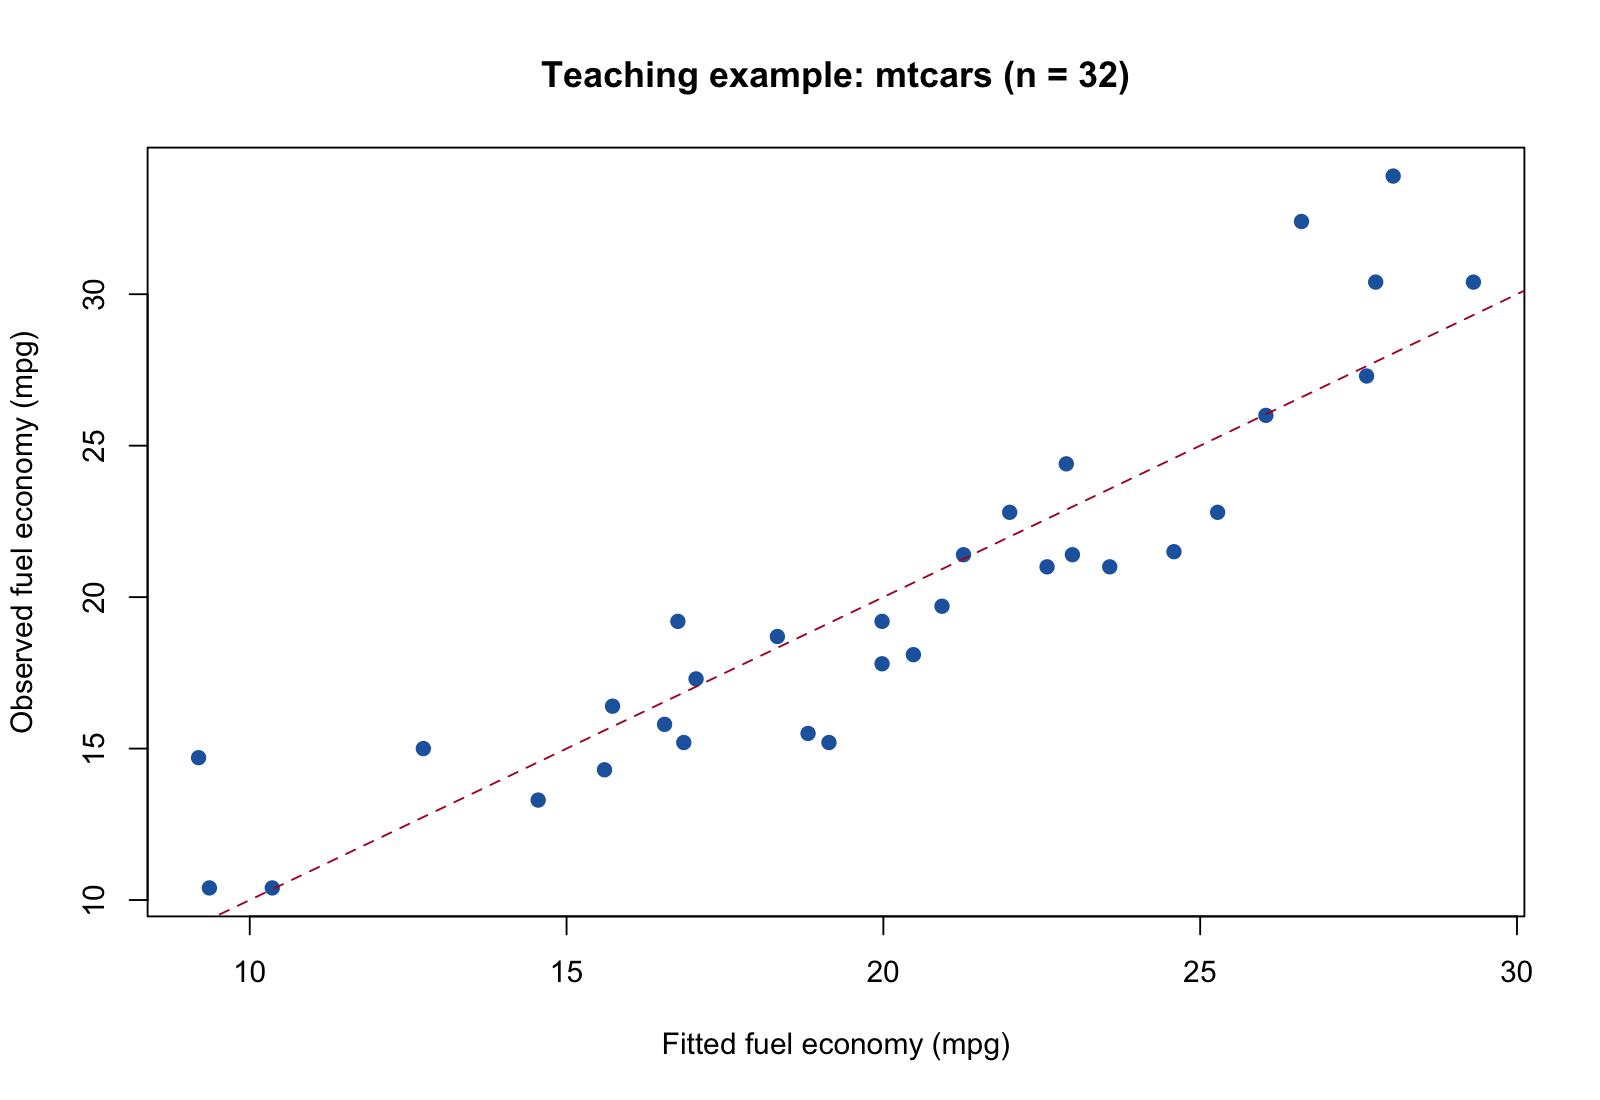
\includegraphics[width=0.82\textwidth]{../../../outputs/figures/observed-fitted.pdf}
  \caption{观测值与拟合值。PDF 图片由 R 自动生成。}
  \label{fig:observed-fitted}
\end{figure}

\begin{table}[htbp]
  \centering
  \caption{由 R 自动生成的回归系数。}
  \label{tab:coefficients}
  \begin{tabular}{lrrrr}
\hline
Term & Estimate & SE & 95\% CI & $p$ \\
\hline
Intercept & 37.227 & 1.599 & [33.957, 40.497] & $<0.001$ \\
Weight (1000 lbs) & -3.878 & 0.633 & [-5.172, -2.584] & $<0.001$ \\
Horsepower & -0.032 & 0.009 & [-0.050, -0.013] & 0.001 \\
\hline
\end{tabular}

\end{table}

图~\ref{fig:observed-fitted}与表~\ref{tab:coefficients}均使用相对路径。
改变 R 分析并重新构建论文后，两者会同步更新。

\section{局限}

这个小型观察性示例用于演示文件流程，不支持因果推断。正式分析仍需检查
模型诊断并提供专业背景依据。

\bibliographystyle{imsart-nameyear}
\bibliography{references}

\end{document}
